\documentclass[11pt,a4paper]{article}

\usepackage[utf8]{inputenc}
\usepackage[T1]{fontenc}
\usepackage[english]{babel}
\usepackage{lmodern}

\usepackage{geometry}
\geometry{
    top=2.5cm,
    bottom=2.5cm,
    left=2.5cm,
    right=2.5cm
}

\usepackage{amsmath,amssymb}
\usepackage{booktabs}
\usepackage{array}
\usepackage{graphicx}
\usepackage{listings}
\usepackage{xcolor}
\usepackage{fancyhdr}
\usepackage{hyperref}

\pagestyle{fancy}
\fancyhf{}
\rhead{\textit{Practical 3: Visualisation using qplot()}}
\lhead{\textit{Data Science --- ETSINF (UPV)}}
\cfoot{\thepage}

\lstset{
    language=R,
    basicstyle=\ttfamily\footnotesize,
    keywordstyle=\color{blue}\bfseries,
    commentstyle=\color{gray}\itshape,
    stringstyle=\color{teal},
    numbers=none,
    frame=lines,
    breaklines=true,
    breakatwhitespace=true,
    showstringspaces=false,
    captionpos=b,
    tabsize=2
}

\title{\textbf{Practical 3: Visualisation using \texttt{qplot()}}\\[0.4ex] \Large Data Science (CDA) --- Academic Lab Report}
\author{\textbf{Enrique Sopeña} \\ 
Máster Universitari en Enginyeria Informàtica (MUIInf) \\
Escola Tècnica Superior d'Enginyeria Informàtica (ETSINF) \\ 
Universitat Politècnica de València}
\date{\today}

\begin{document}

\maketitle

\begin{abstract}
    This report documents the implementation, graphical validation, and clinical data interpretation of Practical~3 (\textit{Visualisation using \texttt{qplot()}}) for the Data Science curriculum at ETSINF (UPV). Using the \texttt{ggplot2} framework in R, we analyze real-world surgical records from $N=394$ patients diagnosed with keratoconus who underwent intrastromal corneal ring segment (ICRS) implantation. We evaluate corneal topography parameters (primary keratometry $K_1$ and orthogonal curvature $K_2$), post-operative outcomes ($K_{1.\text{output}}$), and surgical design choices (number of rings, incision diameter, and ring thickness). The experimental pipeline covers non-parametric local polynomial smoothing (LOESS), ordinary least squares (OLS) linear regressions, aesthetic mappings, conditional discrete distributions, multi-panel faceting, and interquartile dispersion via boxplots.
\end{abstract}

\vspace{0.8em}
\hrule
\vspace{1em}

\section{Introduction and Clinical Context}
Keratoconus is a progressive non-inflammatory ectatic corneal dystrophy characterized by localized thinning and biomechanical weakening of corneal collagen fibrils. This structural degeneration induces a conical protrusion of the optical dome, yielding severe irregular astigmatism, high-order visual aberrations, and significant visual acuity loss.

One prominent conservative surgical intervention consists of the placement of intrastromal corneal ring segments (ICRS). These polymethyl methacrylate (PMMA) micro-segments induce an arc-shortening mechanical effect across the corneal lamellae, producing an intentional biomechanical flattening and reshaping of the anterior curvature. The dataset \texttt{Queratocono.csv} compiles clinical pre-operative measurements, surgical procedure specifications, and post-operative evaluations for 394 treated eyes across 16 numerical and categorical features.

% -------------------------------------------------------------
\section{Exercise 1: Curvature Relation ($K_1$ vs.\ $K_2$) with Smoother}

\subsection{Objective and Implementation}
The objective is to explore the baseline anatomical dependency between the principal meridian curvature ($K_1$) and its orthogonal counterpart ($K_2$), contrasting non-parametric local polynomial regression (LOESS) against parametric linear modeling (ordinary least squares).

\begin{lstlisting}
library(ggplot2)
queratocono <- read.csv("dataset/Queratocono.csv", header = TRUE, sep = ",", check.names = TRUE)

# 1.a) Default non-parametric smoother (LOESS)
p1_loess <- qplot(K1, K2, data = queratocono, geom = c("point", "smooth"))

# 1.b) Parametric linear regression smoother (method = "lm")
p1_lm <- qplot(K1, K2, data = queratocono, geom = c("point", "smooth"), method = "lm")
\end{lstlisting}

\subsection{Graphical Evaluation and Discussion}
\begin{figure}[htbp]
    \centering
    \begin{minipage}{0.48\textwidth}
        \centering
        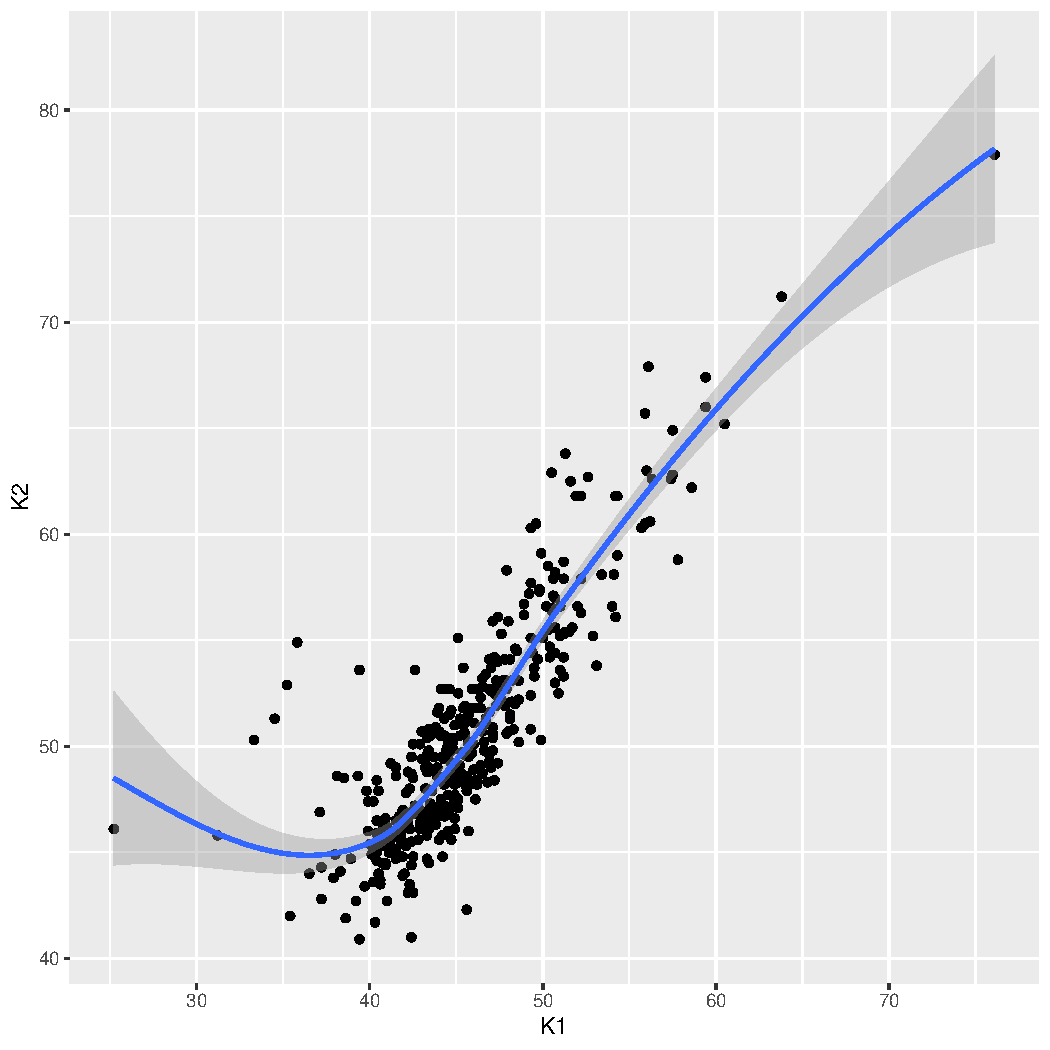
\includegraphics[width=\textwidth,page=1]{../Rplots.pdf}
        \caption{Default LOESS smoother on $K_1$ vs.\ $K_2$.}
        \label{fig:ex1_loess}
    \end{minipage}\hfill
    \begin{minipage}{0.48\textwidth}
        \centering
        \includegraphics[width=\textwidth,page=2]{../Rplots.pdf}
        \caption{Linear model fit (\texttt{method = "lm"}).}
        \label{fig:ex1_lm}
    \end{minipage}
\end{figure}

The LOESS smoother (Figure~\ref{fig:ex1_loess}) reveals a non-linear curvature flattening below $K_1 < 40$ diopters, transitioning into a strong linear regime across the bulk of the patient cohort ($40 \le K_1 \le 60$). At the extreme upper bound ($K_1 > 60$), the 95\% confidence envelope widens significantly due to sample sparsity in severe advanced ectasias. Conversely, the OLS linear model (Figure~\ref{fig:ex1_lm}) imposes a constant slope throughout the domain ($K_2 \approx \beta_0 + \beta_1 K_1$), confirming strong overall collinearity ($r > 0.85$) while obscuring localized deviations at low curvature boundaries.

% -------------------------------------------------------------
\section{Exercise 2: Keratometric Relationship Stratified by Ring Count}

\subsection{Objective and Implementation}
We assess whether the morphological relationship between $K_1$ and $K_2$ exhibits structural divergence conditional on the surgical decision to implant either one or two rings (\texttt{na} $\in \{1, 2\}$).

\begin{lstlisting}
p2 <- qplot(K1, K2, 
            data = queratocono, 
            colour = factor(na), 
            geom = c("point", "smooth"), 
            method = "lm", 
            main = "Relation between K1 and K2")
\end{lstlisting}

\subsection{Graphical Evaluation and Discussion}
\begin{figure}[htbp]
    \centering
    \includegraphics[width=0.62\textwidth,page=3]{../Rplots.pdf}
    \caption{Stratified linear regressions for $K_1$ vs.\ $K_2$ by factor(\texttt{na}).}
    \label{fig:ex2}
\end{figure}

Mapping \texttt{colour = factor(na)} instructs \texttt{qplot()} to partition the regression estimator across levels 1 and 2 independently:
\begin{itemize}
    \item \textbf{Single-ring implants (\texttt{na = 1}, red):} Patients receiving a single ring segment present a slightly steeper slope and higher dispersion in advanced curvatures, often corresponding to asymmetrical, highly localized inferior cones.
    \item \textbf{Double-ring implants (\texttt{na = 2}, blue/cyan):} Concentrated along a tighter trajectory, reflecting central, symmetric keratoconic cones where dual segments are indicated to achieve uniform circumferential flattening.
\end{itemize}

% -------------------------------------------------------------
\section{Exercise 3: Pre-operative vs.\ Post-operative Curvature}

\subsection{Objective and Implementation}
The surgical efficacy of the procedure is evaluated by confronting pre-operative principal keratometry ($K_1$) with post-operative principal keratometry ($K_{1.\text{output}}$).

\begin{lstlisting}
p3 <- qplot(K1, K1.salida, data = queratocono, geom = "point")
\end{lstlisting}

\subsection{Graphical Evaluation and Discussion}
\begin{figure}[htbp]
    \centering
    \includegraphics[width=0.58\textwidth,page=4]{../Rplots.pdf}
    \caption{Pre-operative ($K_1$) vs.\ post-operative ($K_{1.\text{output}}$) corneal curvature.}
    \label{fig:ex3}
\end{figure}

The scatter plot exhibits an extremely tight linear correlation, demonstrating predictable surgical predictability across the sample. Most data points lie below the theoretical identity line $y = x$, visually confirming the desired flattening effect ($K_{1.\text{output}} < K_1$). Two notable clinical outliers are detected: an isolated patient displaying exceptional pre-operative steepness ($K_1 > 75$, remaining near $45$ diopters post-operatively) and an atypical measurement near $K_1 \approx 64$ with $K_{1.\text{output}} \approx 63$, indicating a candidate refractory to standard flattening.

% -------------------------------------------------------------
\section{Exercise 4: Distribution of Ring Thickness by Segment Count}

\subsection{Objective and Implementation}
The frequency profile of ring thickness (\texttt{grosor}, in $\mu$m) is analyzed as a discrete factor, with the bar fill stacked according to segment count (\texttt{na}).

\begin{lstlisting}
p4 <- qplot(factor(grosor), data = queratocono, geom = "bar", fill = factor(na))
\end{lstlisting}

\subsection{Graphical Evaluation and Discussion}
\begin{figure}[htbp]
    \centering
    \includegraphics[width=0.58\textwidth,page=5]{../Rplots.pdf}
    \caption{Stacked bar chart of factor(\texttt{grosor}) partitioned by factor(\texttt{na}).}
    \label{fig:ex4}
\end{figure}

The empirical distribution indicates marked clinical preference for $200\,\mu\text{m}$ ($n=179$) and $250\,\mu\text{m}$ ($n=127$) rings. Intermediate thicknesses ($175\,\mu\text{m}$, $225\,\mu\text{m}$, $275\,\mu\text{m}$) are deployed exclusively in dual-ring configurations (\texttt{na = 2}), where asymmetric combinations of different thicknesses are paired to correct asymmetrical astigmatic components.

% -------------------------------------------------------------
\section{Exercise 5: Multi-dimensional Faceting by Incision Diameter and Rings}

\subsection{Objective and Implementation}
We examine high-dimensional interactions by conditioning the $K_1$--$K_2$ relationship across surgical incision diameter (\texttt{diam} $\in \{5, 6\}\,\text{mm}$, row panels) and segment count (\texttt{na} $\in \{1, 2\}$, column panels), encoding ring thickness via color and mitigating point occlusion through an alpha transparency of $1/3$.

\begin{lstlisting}
p5 <- qplot(K1, K2, 
            data = queratocono, 
            facets = diam ~ na, 
            colour = factor(grosor), 
            alpha = I(1/3))
\end{lstlisting}

\subsection{Graphical Evaluation and Discussion}
\begin{figure}[htbp]
    \centering
    \includegraphics[width=0.68\textwidth,page=6]{../Rplots.pdf}
    \caption{Faceted scatter plot ($2 \times 2$ grid: \texttt{diam $\sim$ na}) with alpha blending.}
    \label{fig:ex5}
\end{figure}

The faceting grid elucidates surgical protocol segmentation:
\begin{itemize}
    \item Smaller optical diameter ($5\,\text{mm}$, top row) is predominantly chosen for eyes with moderate keratometry, providing stronger focal refractive flattening closer to the visual axis.
    \item Larger diameter ($6\,\text{mm}$, bottom row) exhibits broader corneal coverage, accommodating eyes with steeper baseline deformities.
    \item The transparency factor $\alpha = 1/3$ effectively reveals point density clusters around $K_1 \in [42, 48]$ and prevents misinterpretation of high-density overlap regions.
\end{itemize}

% -------------------------------------------------------------
\section{Exercise 6: Distributional Summaries via Boxplots}

\subsection{Objective and Implementation}
To assess median curvature progression and interquartile dispersion across segment thicknesses, independent box-and-whisker plots are constructed for both corneal axes.

\begin{lstlisting}
p6_k1 <- qplot(factor(grosor), K1, data = queratocono, geom = "boxplot")
p6_k2 <- qplot(factor(grosor), K2, data = queratocono, geom = "boxplot")
\end{lstlisting}

\subsection{Graphical Evaluation and Discussion}
\begin{figure}[htbp]
    \centering
    \begin{minipage}{0.48\textwidth}
        \centering
        \includegraphics[width=\textwidth,page=7]{../Rplots.pdf}
        \caption{Boxplot of $K_1$ across \texttt{factor(grosor)}.}
        \label{fig:ex6_k1}
    \end{minipage}\hfill
    \begin{minipage}{0.48\textwidth}
        \centering
        \includegraphics[width=\textwidth,page=8]{../Rplots.pdf}
        \caption{Boxplot of $K_2$ across \texttt{factor(grosor)}.}
        \label{fig:ex6_k2}
    \end{minipage}
\end{figure}

Across both axes, median keratometric steepness rises monotonically with ring thickness: eyes requiring thicker rings ($225\,\mu\text{m}$ to $300\,\mu\text{m}$) exhibit higher baseline disease stages. The $200\,\mu\text{m}$ category shows the highest number of positive upper outliers ($K_1, K_2 > 65$), reflecting its status as the most versatile standard choice across diverse disease profiles.

% -------------------------------------------------------------
\newpage
\appendix
\section*{Appendix: Complete Sequential Execution Log}
\addcontentsline{toc}{section}{Appendix: Complete Sequential Execution Log}

The verbatim console output recorded during the sequential execution of \texttt{pract3.R} is reproduced below:

\begin{lstlisting}[language={}, basicstyle=\ttfamily\scriptsize, frame=single, breaklines=true]
'data.frame':	394 obs. of  16 variables:
 $K1       : num  38.1 39.4 43.3 45.7 44.6 44.2 44.2 53.1 45.1 40.7 ...$ K2       : num  48.6 53.6 50.4 50.1 50.4 44.8 45.8 53.8 52.5 44.5 ...
 $ch       : num  6.9 5.7 8.8 11.1 11.1 8.9 11.1 7.5 7.7 9.4 ...$ na       : int  2 2 2 1 2 1 1 1 2 1 ...
 $Incision : int  60 140 120 30 60 180 130 60 60 30 ...$ Prof     : int  390 400 381 370 440 327 380 400 380 477 ...
 $diam     : int  5 5 5 5 5 6 6 5 6 5 ...$ grosor   : int  300 300 200 250 200 200 200 200 225 200 ...
 $Longitud1: int  90 105 120 160 120 150 210 160 120 160 ...$ Longitud2: int  180 210 240 160 240 150 210 160 240 160 ...
 $grosor1  : int  300 300 200 250 200 200 200 200 200 200 ...$ grosor2  : int  300 300 200 0 200 0 0 0 250 0 ...
 $long1    : int  90 90 120 160 120 150 210 160 90 160 ...$ long2    : int  90 120 120 0 120 0 0 0 150 0 ...
 $K1.salida: num  35.5 42 42.7 45.8 44.4 42.8 43.1 48.7 45.7 39.8 ...$ Astig    : num  10.1 8.9 3 1.9 2.9 2.3 3.9 2.8 3.2 3.8 ...
    K1   K2   ch na Incision Prof diam grosor Longitud1 Longitud2 grosor1
1 38.1 48.6  6.9  2       60  390    5    300        90       180     300
2 39.4 53.6  5.7  2      140  400    5    300       105       210     300
3 43.3 50.4  8.8  2      120  381    5    200       120       240     200
4 45.7 50.1 11.1  1       30  370    5    250       160       160     250
5 44.6 50.4 11.1  2       60  440    5    200       120       240     200
6 44.2 44.8  8.9  1      180  327    6    200       150       150     200
  grosor2 long1 long2 K1.salida Astig
1     300    90    90      35.5  10.1
2     300    90   120      42.0   8.9
3     200   120   120      42.7   3.0
4       0   160     0      45.8   1.9
5     200   120   120      44.4   2.9
6       0   150     0      42.8   2.3
Warning message:
`qplot()` was deprecated in ggplot2 3.4.0. 
`geom_smooth()` using method = 'loess' and formula = 'y ~ x'
`geom_smooth()` using method = 'loess' and formula = 'y ~ x'
pdf 
  2 
Warning message:
In geom_point(method = "lm") : Ignoring unknown parameters: `method`
`geom_smooth()` using formula = 'y ~ x'
`geom_smooth()` using formula = 'y ~ x'
pdf 
  2 
Warning message:
In geom_point(method = "lm") : Ignoring unknown parameters: `method`
`geom_smooth()` using formula = 'y ~ x'
`geom_smooth()` using formula = 'y ~ x'
pdf 
  2 
pdf 
  2 
pdf 
  2 
pdf 
  2 
pdf 
  2 
pdf 
  2 
\end{lstlisting}

\end{document}